%==============================================================================
\chapter{A CCM Overview}
%==============================================================================
\begin{flushright}
{\it }
\end{flushright}

%==============================================================================
\section{Introduction}
%==============================================================================
The {\it Object Management Group} (OMG) has been standardizing an open
middleware specification to support distributed applications. The OMG specified
an sophisticated component model based on the {\it Common Object Request Broker
Architecture} (CORBA) called {\it CORBA Component Model} (CCM)
\cite{CCMSpecification}.



%==============================================================================
\section{Component model}
%==============================================================================

The CCM defines a component architecture and a container framework in which the
component life cycle takes place.
\begin{figure}[htbp]
    \begin{center}
        \includegraphics [width=6cm,angle=0] {Component}
        \caption{CCM component}
        \label{component}
    \end{center}
\end{figure}

A {\it CCM Component} (Fig.~\ref{component}) provides a variety of surface
features that support ways to connect components together to form assemblies:
\begin{description}
\item [Home]
The component home is an interface that defines factory and finder methods to
create or find component instances managed by the home. Each home supports at
least one {\tt create} method.

\item [Equivalent interface]
Every IDL3 interface (containing the keywords {\tt component}, {\tt home}, etc.)
will be transformed into a classic IDL interface that can be processed by a
regular IDL compiler -- the equivalent interface. This IDL3 to IDL mapping adds
some interfaces and equivalent operations to the user written interfaces. As
described by the CCM specification, every IDL3 construct defines its
 own IDL3 to IDL mapping.

\item [Supported interface]
A home or component definition can support zero or more interfaces that results
in inheritance of supported interfaces in the corresponding equivalent
interfaces.

\item [Attribute] 
Component or a component home can have attributes that are named values exposed
through accessor and mutator operations. Attributes are primarily intended to be
used for component configuration.

\item [Facet] 
A component's facet is a named interface that provides access to specific
component methods. A component may have zero ore more facets. The component's
equivalent interface inherits the {\tt Components::Navigation} interface that
defines generic operations for facet access.

\item [Receptacle]
A component's receptacle is an abstraction that is concretely manifested on a
component as a set of operations for establishing and managing connections. A
component may have zero ore more receptacles. The component's equivalent
interface inherits the {\tt Components::Receptacles} interface that defines
generic operations for receptacle management.

\item [Event source] 
An event source embodies the potential for the component to generate events of a
specified type and provides mechanisms for associating consumers with sources.
There are two categories of event sources, {\it emitters} and {\it publishers}.
An emitter can be connected to at most one proxy provider by the container. A
publisher can be connected through the channel to an arbitrary number of
consumers that are subscribed to the publisher event source.

\item [Event sink] 
An event sink embodies the potential for the component to receive events of a
specified type.
\end{description}

The component model is also defined in a MOF compliant metamodel, the {\it
Interface Repository Metamodel}, that expresses the extensions to classic IDL
defined by the CCM.

%==============================================================================
\section{Component container}
%==============================================================================

Components run in a {\it CCM Container} (Fig.~\ref{container}) that provides the
runtime environment for CORBA components. Containers are built on the {\it
Object Request Broker} (ORB), the {\it Portable Object Adapter} (POA) and CORBA
services.

\begin{figure}[htbp]
    \begin{center}
        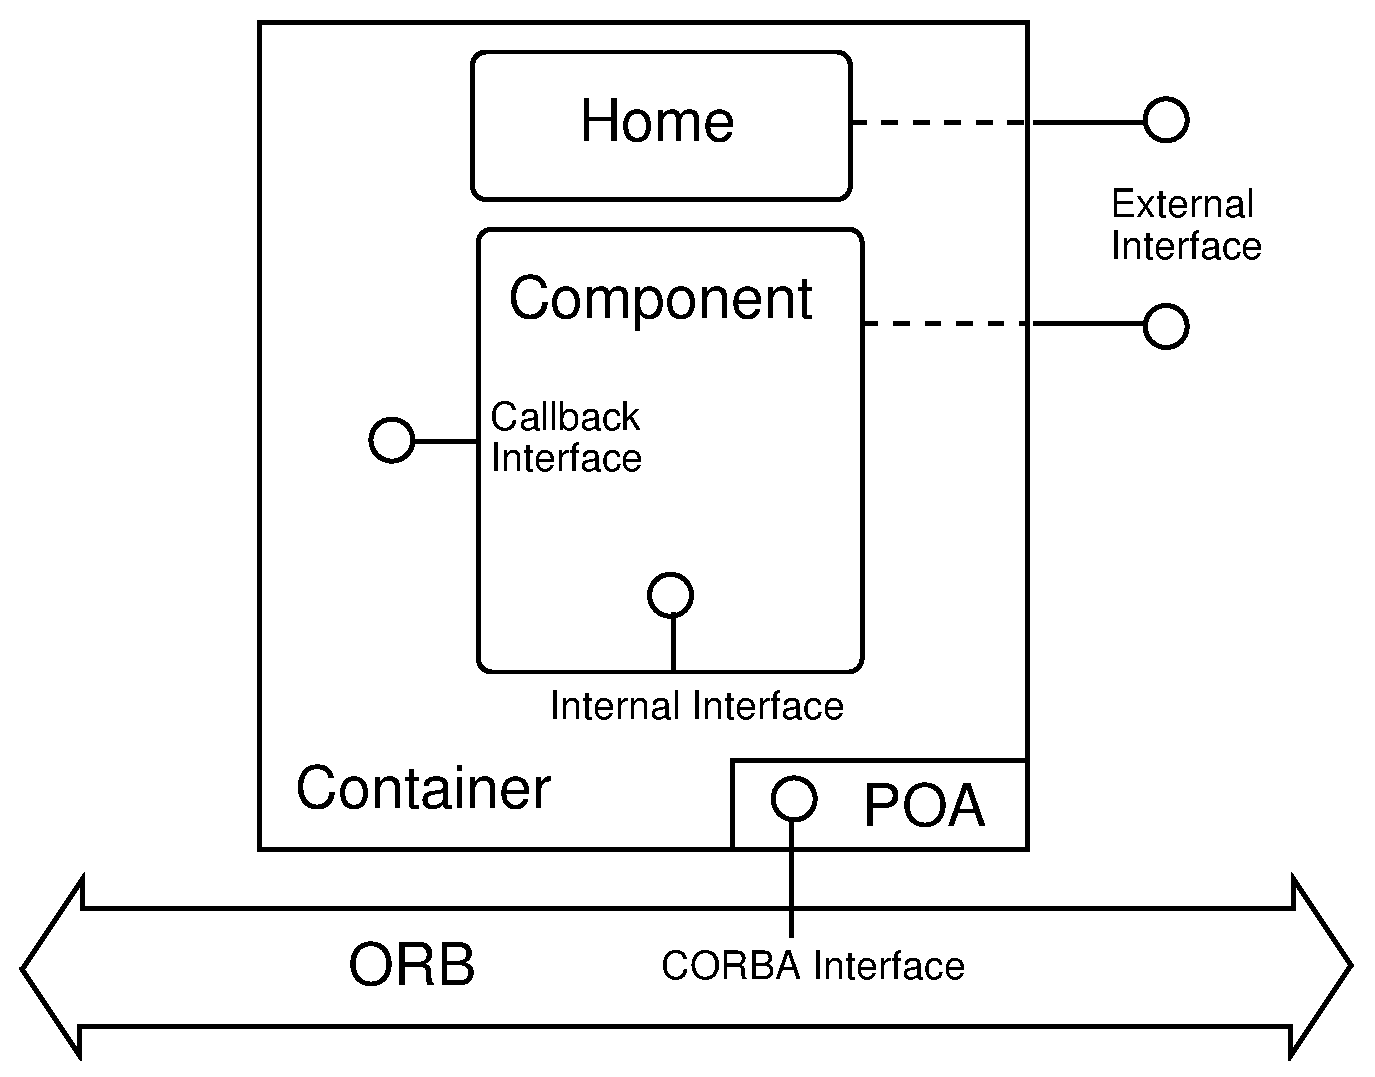
\includegraphics [width=6cm,angle=0] {Container}
        \caption{CCM container}
        \label{container}
    \end{center}
\end{figure}

As shown in Fig.~\ref{container}, the container programming model is made of the
following interfaces that are used by the client, the container and the
components:
\begin{description}
\item [Internal interfaces]
These local interfaces are used by the component developer and provided by the
container to assist in the implementation of the component's behavior.

\item [External interfaces]
The external interfaces define the external view of a component. They are used
by the client and implemented by the component developer.

\item [Callback interfaces]
These local interfaces are used by the container and implemented by the
component, either in generated code or directly, in order for the component to
be deployed in the container.
\end{description}


The CCM specification defined component categories whose behavior is specified
by the two container API types. Additionally there is a component category that
describe the empty container.
\begin{description}
\item [Service component]
The service component has behavior, no state and no identity. The lifespan of a
service component is equivalent to the lifetime of a single operation request.

\item [Session component]
The session component has behavior, transient state and a identity that is not
persistent. Note that the session component is equivalent to the stateful
session bean found in EJB.

\item [Process component]
The process component has behavior, persistent state which is not visible to the
client, and a persistent identity.

\item [Entity component]
The entity component has behavior, persistent state which is visible to the
client, and a identity which is visible to the clients through a primary key
declaration.


\end{description}



%==============================================================================
\section{Component assembly}
%==============================================================================

Connecting components by their ports leads to component {\it Assemblies} as
shown in Fig.~\ref{assemblygraph}.

\begin{figure}[htbp]
    \begin{center}
        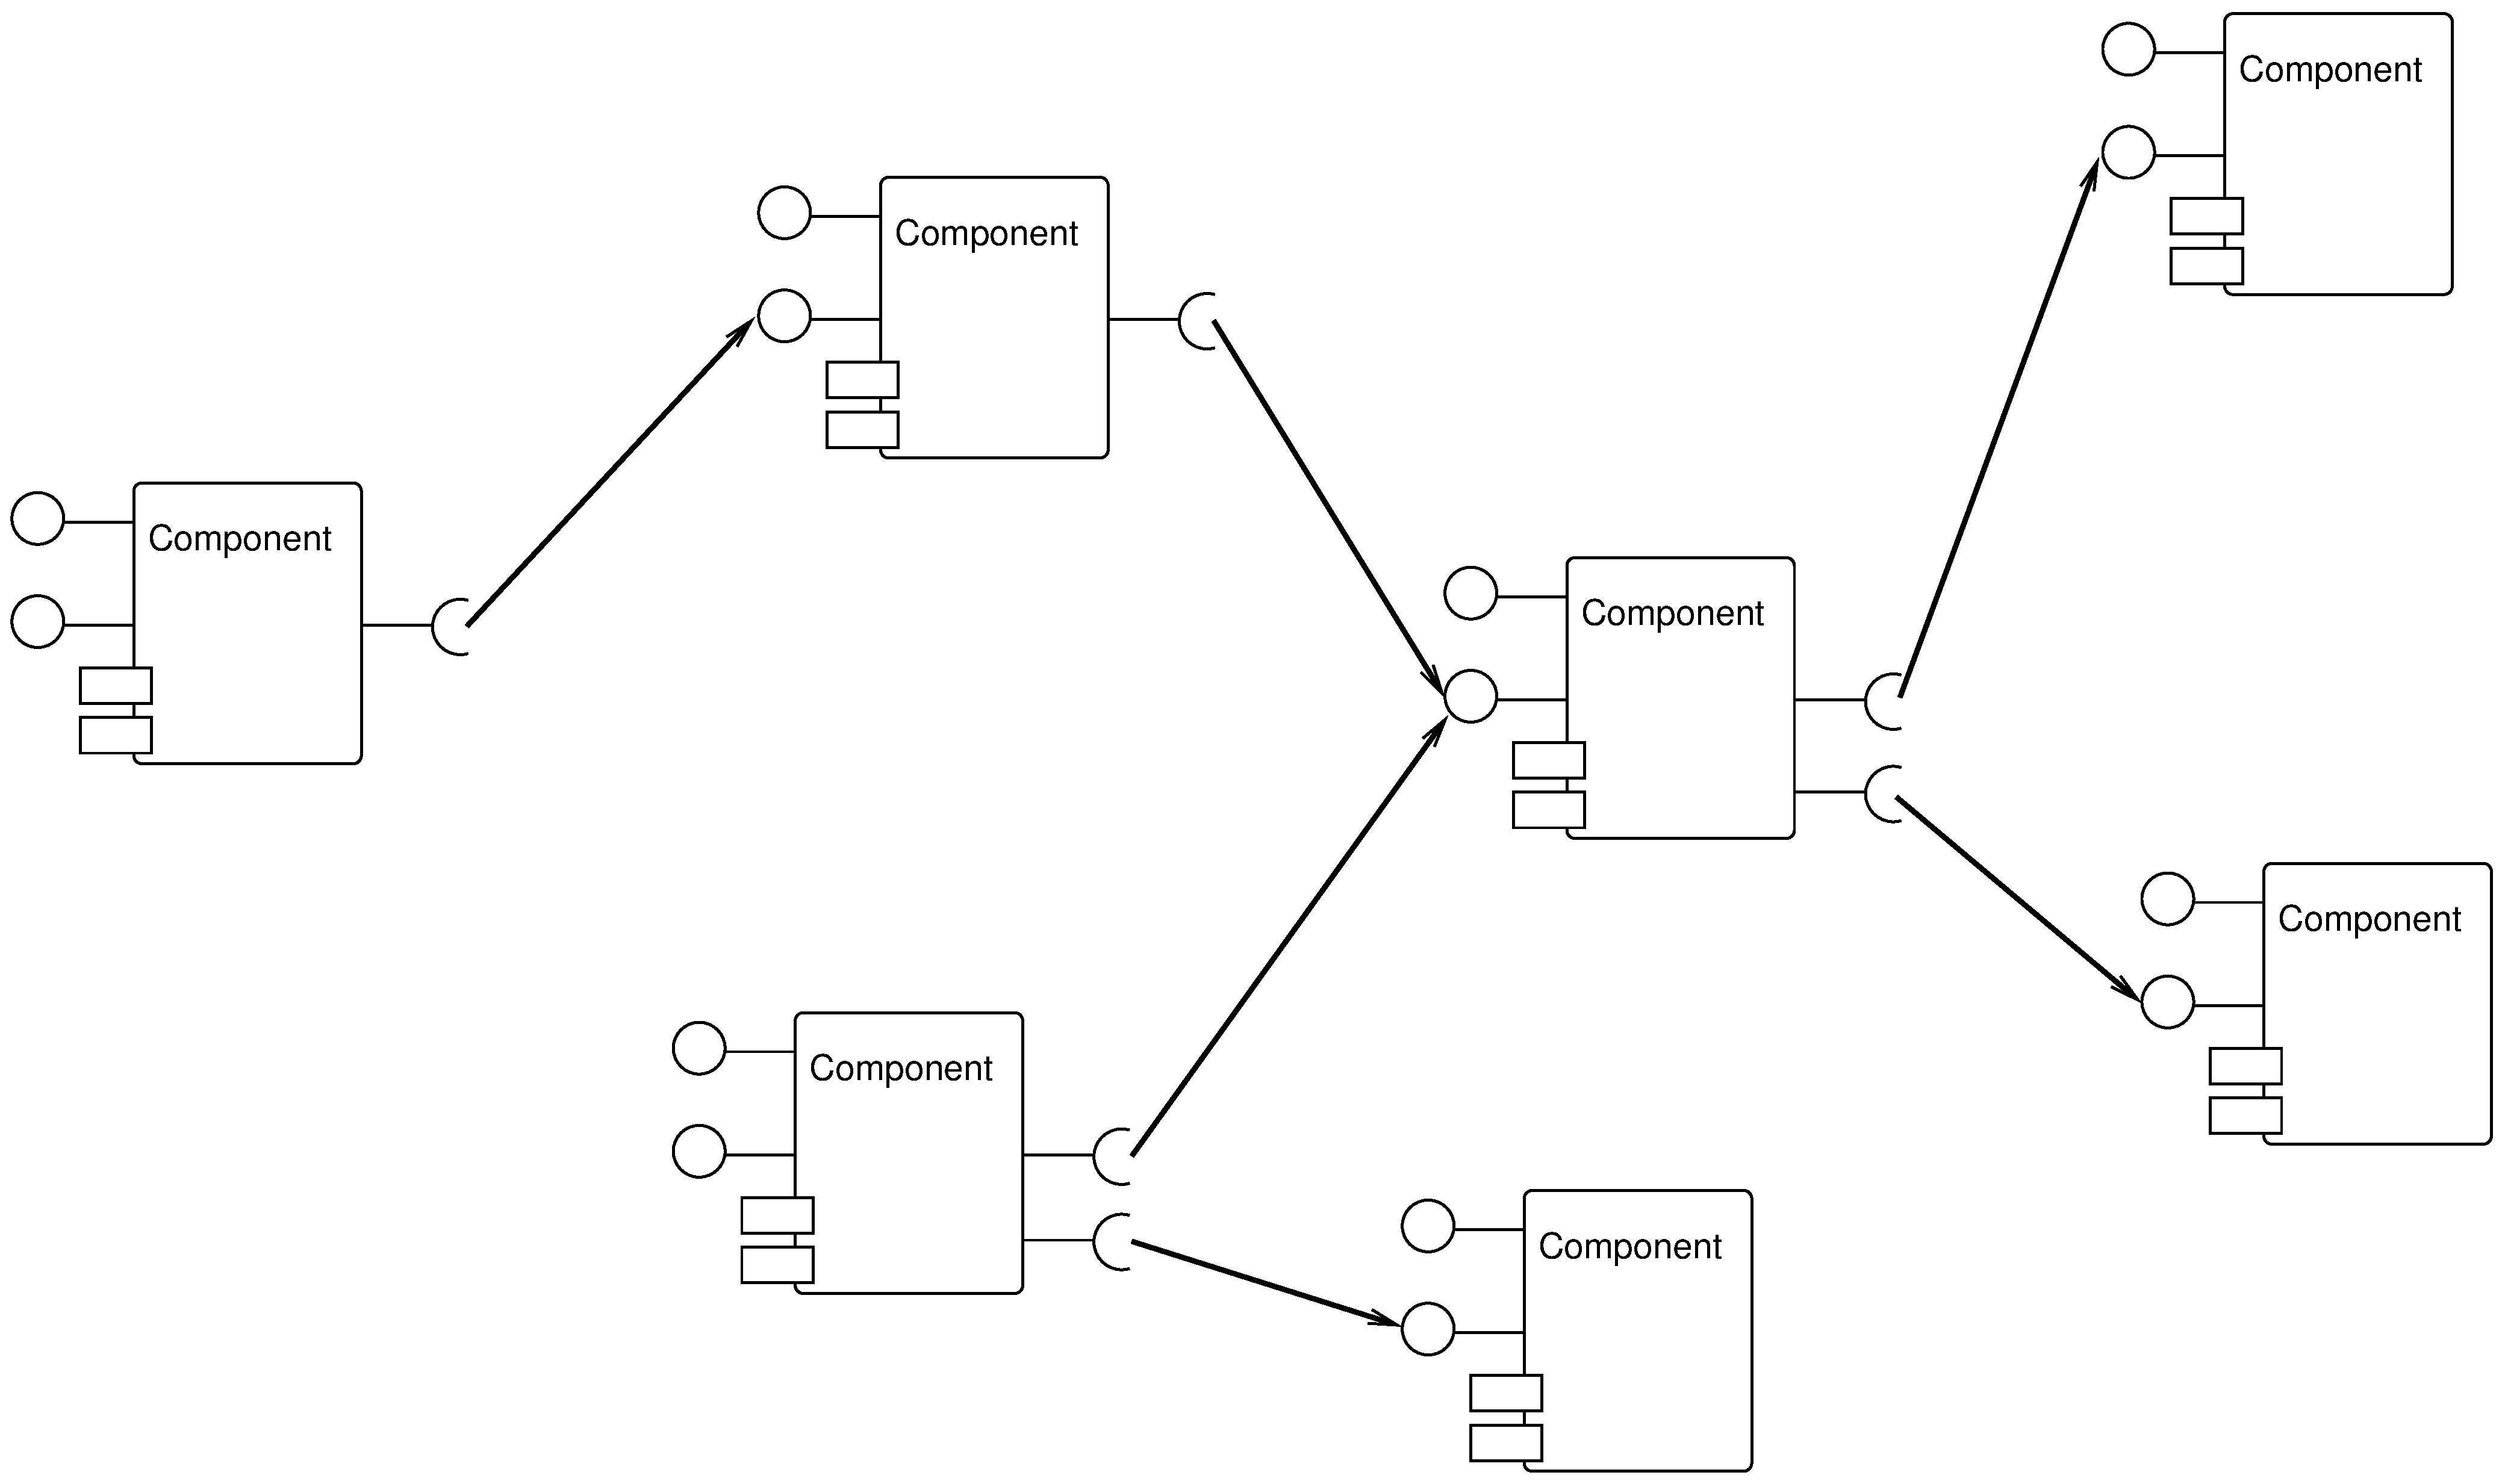
\includegraphics [width=6cm,angle=0] {Assembly.eps}
        \caption{Component assembly}
        \label{assemblygraph}
    \end{center}
\end{figure}

The CCM specification defines an {\tt Components::Assembly} interface that
represents an assembly instantion. It is used to build up and tear down
component assemblies. Building the assembly up means creating all of the
components and establish connections between them as specified in the assembly
descriptor. Tearing the assembly down means removing all connections and
destroying the components.





%==============================================================================
\section{Descriptor files}
%==============================================================================

The CCM specification defines a bunch of XML descriptor files that are used to
describe software packages, components, properties and assemblies.
\begin{description}
\item [Software package descriptor (*.csd)] 
The software package descriptor consists of general information about the
software followed by one or more sections describing implementations of
software.

\item [CORBA component descriptor (*.ccd)]
The component descriptor specifies component characteristics that a design tool
my use to display information about a component (e.g. supported interfaces,
inherited components, used and provided ports, etc.).

\item [Component assembly descriptor (*.cad)]
The assembly descriptor consists of elements describing the components used in
the assembly, connection information and partitioning information.

\item [Property file descriptor (*.cpf)]
The property file is used at deployment time to configure a home or a component
instance. A configurator uses the property file to determine how to set
component and home property attributes.
\end{description}




%==============================================================================
\section{Client programming model}
%==============================================================================

The client interacts with a CORBA component through two forms of external
interfaces, a home interface and one or more application interfaces. Two forms
of clients are supported by the CCM specification:
\begin{description}
\item [Component--aware client] 
This client knows that it is making requests against a component. The client can
use component mechanisms like navigation between component and facets etc.
Component--aware clients locates their interfaces using the {\tt
Components::HomeFinder} or a naming service.\\ A reference that supports the
{\tt HomeFinder} interface may be obtained from the ORB by invoking {\tt
CORBA::ORB::resolve\_initial\_references()} with the parameter value {\tt
``ComponentHomeFinder''}.

\item [Component--unaware client]
This client does not know that there is a CORBA component, the client requests
to ordinary CORBA objects and object factories.
\end{description}



